\documentclass{article}

\usepackage[margin=1in]{geometry}
\usepackage{fancyhdr}
\usepackage{amsmath}
\usepackage{amssymb}
\usepackage{listings}
\usepackage{graphicx}
\usepackage{enumerate}
\usepackage{tikz}
\usetikzlibrary{automata,positioning}


\pagestyle{fancy}

\lhead{CS 373 \\ Homework 3}
\chead{}
\rhead{Drew Cross (ddcross2) \\ \emph{partners}: Eric Parsons \\Bryan Plummer}
\lfoot{}
\cfoot{}
\rfoot{}

\begin{document}

\subsection*{Problem 1}
Prove that the following languages are non-regular using the Myhill-Nerode theorem.
\begin{enumerate}[(a)]

\item $A = \{ww\ |\ w \in \Sigma^*\}$ over the alphabet $\Sigma = \{0,1\}$. (5 Points)

\textbf{Claim:}
    $A = \{ww\ |\ w \in \Sigma^*\}$ over the alphabet $\Sigma = \{0,1\}$ is nonregular.\\
\textbf{Proof:}
    Consider the equivalence relation $\sim_A$ on $A$ and the set of strings \\
    $S = \{10^n | n \geq 0 \}$ \\
    For $x = 10^i$ and $y = 10^j$ where $i \neq j$, \\
    Notice that $\exists z = 10^i$ S.T. $xz \in A$ but
    $yz \notin A$ \\
    Thus $x$ and $y$ belong to separate equivalence classes,
    and each equivalence class for a string in
    $A$ is distinct from the others. Since $S$ is infinite, there must be an infinite number of
    equivalence classes, implying that $A$ is nonregular by the Myhill-Nerode theorem.
    \[ \square \]

\item $B = \{w \in \Sigma^*\ |\ \#0(w) = 2 $ or $ \#2(w) < \#0(w)\}$ over the alphabet
    $\Sigma = \{0,1,2\}$. (5 Points)

\textbf{Claim:}
    $B = \{w \in \Sigma^*\ |\ \#0(w) = 2 $ or $ \#2(w) < \#0(w)\}$ over the alphabet
    $\Sigma = \{0,1,2\}$ is nonregular.\\
\textbf{Proof:}
    Consider the equivalence relation $\sim_B$ on $B$ and the set of strings \\
    $S = \{0^n | n \geq 0 \}$ \\
    For $x = 00^i$ and $y = 00^j$ and $i \neq j$ Without the loss of generality assume
    $i > j$.\footnote{If $i < j$ then $xz \notin B$ and $yz \in B$}\\
    Notice that $\exists z=2^i$ S.T. $xz \in B$ but $yz \notin B$. \\
    Thus $x$ and $y$ belong to separate equivalence classes,
    and each equivalence class for a string in
    $B$ is distinct from the others. Since $S$ is infinite, there must be an infinite number of
    equivalence classes, implying that $B$ is nonregular by the Myhill-Nerode theorem.
    \[ \square \]

\item $C = \{x=y+z | x,y,z$ are natural numbers base 10, and $x$ is the sum of $y$ and $z\}$
    over the alphabet $\Sigma = \{0,1,2,3,4,5,6,7,8,9,+,=\}$. For example, the string
    "15=4+11" is in $C$, but "5=2+2" and "3=3" are not. (5 Points)

\textbf{Claim:}
    $C = \{x=y+z\ |\ x,y,z$ are natural numbers base 10, and $x$ is the sum of $y$ and $z\}$
    is nonregular.
\textbf{Proof:}
    Consider the equivalence relation $\sim_C$ on $C$ and the set of strings \\
    $S = \{ 10^{2n}1 = 1+10^n | n \geq 1\}$
    For $x = 10^{2i}1 = 1 + 10^i \in S$ and $y = 10^{2j} + 10^j \in S$ \\
    Notice there is a string $z = 0^{i+1}$ such that $xz \in S$ but $yz \notin S$ \\
    Thus $x$ and $y$ belong to separate equivalence classes,
    and each equivalence class for a string in
    $B$ is distinct from the others. Since $S$ is infinite, there must be an infinite number of
    equivalence classes, implying that $B$ is nonregular by the Myhill-Nerode theorem.
    \[ \square \]


\end{enumerate}

\newpage


\subsection*{Problem 2}
In a context-free grammar $G = (V, \Sigma, R, S)$, a variable $A \in V$ is called cyclic if for some $u,v \in
(V \cup \Sigma)^*$ there exists a sequence of derivations $A \Rightarrow w_1 \Rightarrow w_2 \Rightarrow$ ... 
$ \Rightarrow w_k \Rightarrow uAv,k \geq 0$. Grammar $G$ is cyclic if at least one of its variables is cyclic,
otherwise $G$ is cycle-free.
\begin{enumerate}[(a)]
\item Prove that the language generated by a cycle-free grammar is finite. (10 Points)

A Language generated by a cycle-free grammar is finite because a grammar contains a finite
number of rules. Because there are no cycles, we can take one of the derivations for the start state
and replace each variable on the right side with its production. We can now "push down" the chosen
variable into each of the other rules. Since there are no cycles, we can do this for each variable
until we are left with terminals only. If there were cycles we would find a point where "pushing
down" the variables would become futile, because we would just keep expanding the rules
infinitely. Now that we have removed all variables, we have our start variable going to a set of
strings, which exactly describes our language. For example: \\

\begin{minipage}[c]{0.5\linewidth}
$S \rightarrow A\ |\ B$ \\
$A \rightarrow C\ |\ D$ \\
$B \rightarrow E\ |\ A$ \\
$C \rightarrow aa\ |\ bb$ \\
$D \rightarrow a\ |\ b$ \\
$E \rightarrow aba\ |\ bab$ \\
\textbf{Replacing A:}\\
$S \rightarrow C\ |\ D\ |\ B$ \\
$B \rightarrow E\ |\ C\ |\ D$ \\
$C \rightarrow aa\ |\ bb$ \\
$D \rightarrow a\ |\ b$ \\
$E \rightarrow aba\ |\ bab$ \\
\textbf{Replacing C:} \\
$S \rightarrow aa\ |\ bb\ |\ D\ |\ B$ \\
$B \rightarrow E\ |\ aa\ |\ bb\ |\ D$ \\
$D \rightarrow a\ |\ b$ \\
$E \rightarrow aba\ |\ bab$ \\
\end{minipage}
\begin{minipage}[c]{0.5\linewidth}
\textbf{Replacing D:} \\
$S \rightarrow aa\ |\ bb\ |\ a\ |\ b\ |\ B$ \\
$B \rightarrow E\ |\ aa\ |\ bb\ |\ a\ |\ b$ \\
$E \rightarrow aba\ |\ bab$ \\
\textbf{Replacing B:}\\
$S \rightarrow aa\ |\ bb\ |\ a\ |\ b\ |\ E\ |\ aa\ |\ bb\ |\ a\ |\ b$ \\
$E \rightarrow aba\ |\ bab$ \\
\textbf{Replacing E:}\\
$S \rightarrow aa\ |\ bb\ |\ a\ |\ b\ |\ aba\ |\ bab\ |\ aa\ |\ bb\ |\ a\ |\ b$ \\
\end{minipage}

\item Is it necessarily true that the language generated by a cyclic grammar is infinite? Explain your
answer. (5 Points).

No, If a language cycles with only variables and only exits to terminals with no variables.
For example the grammar $A$: \\
$A \rightarrow B $ \\
$B \rightarrow C $ \\
$C \rightarrow A\ |\ ab$



\end{enumerate}

\newpage


\subsection*{Problem 3}
Construct CFGs for the following languages. Give a brief explanation of how your
grammar works and what each nonterminal stands for. The CFGs must be designed
by hand and not converted from PDAs using the equivalence theorem.

\begin{enumerate}[(a)]
\item $A = \{0^m1^n\ |\ m > n \geq 0$ and $ m - n$ is even$\}$. (5 Points)

$S \rightarrow A$ \\
$A \rightarrow 00\ |\ 0A1\ |\ 00A $\\
A here forces $\#_0 > \#_1$ and m-n to be even by only allowing additions of 1's with 0's in
pairs (0A1) and only allowing even additions of 0's otherwise.


\item The compliment of $B = \{0^n1^n | n \geq 0\}$ over the alphabet $\Sigma = \{0,1\}$. (5 Points)

$S \rightarrow\ A\ |\ B\ |\ C10C $ \\
$A \rightarrow\ 0\ |\ 0A\ |\ 0A1 $ \\
$B \rightarrow\ 1\ |\ B1\ |\ 0B1 $ \\
$C \rightarrow\ 0C\ |\ 1C |\ \varepsilon $

A is all strings where we have more 1's than 0's. \\
B is all strings where we have more 0's than 1's \\
C covers all cases where we have a 0 after a 1.

\item $C = \{0^m1^n2^k3^l | m+n=k+l, m,n,k,l \geq 0\}$. (5 Points)

$S \rightarrow 0S3\ |\ B\ |\ C $ \\
$B \rightarrow 0B2\ |\ D $ \\
$C \rightarrow 1C2\ | D $ \\
$D \rightarrow 1D2\ |\ \varepsilon$

Here we need to build strings from the outside in, and we can move in one side at a time
(such as going from S to B, or both at a time (such as going from S to C: \\
S is building the 0's and 3's in pairs. \\
B builds up 0's and 2's together. \\
C builds up 1's and 3's together. \\
D builds up 1's and 2's together and allows for the termination of the strings. Additionally,
from S we can get to B and C, and "drill down" from B or C to D.

\end{enumerate}

\newpage


\subsection*{Problem 4}
Construct PDAs for the following languages and explain how htey work. The PDAs must be designed by hand and
not converted from CFGs using the equivalence theorem.

\begin{enumerate}[(a)]
\item $A = \{ 0^n1^{2n+m}0^{m-1} | m,n \in \mathbb{N}\}$. (5 Points)

    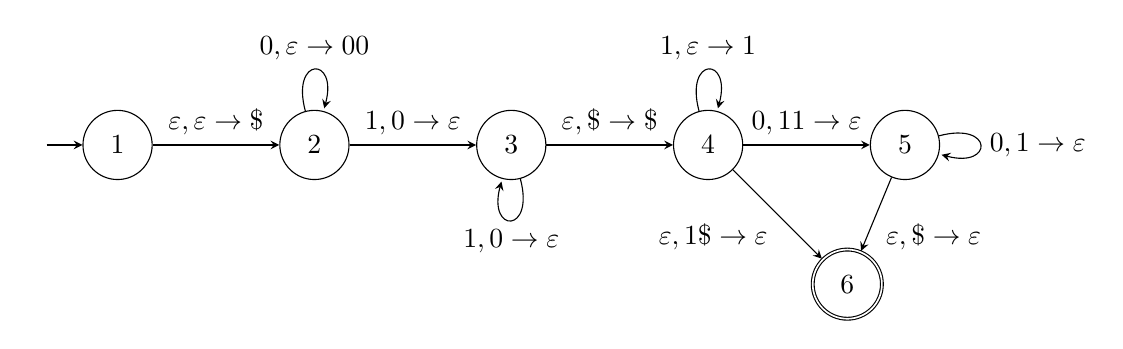
\begin{tikzpicture}[%
    >=stealth,
    node distance=2.5cm,
    on grid,
    auto
    ]

    \node[initial,initial text=,state] (1)  {1};
    \node[state] (2) [right of=1] {2};
    \node[state] (3) [right of=2] {3};
    \node[state] (4) [right of=3] {4};
    \node[state] (5) [right of=4] {5};
    \node[state, accepting] (6) [below right of=4] {6};

    \path[->] (1) edge node {$\varepsilon, \varepsilon \rightarrow \$$} (2);
    \path[->] (2) edge[loop above] node {$0, \varepsilon \rightarrow 00$} (2);
    \path[->] (2) edge node {$1,0 \rightarrow \varepsilon$} (3);
    \path[->] (3) edge[loop below] node {$1,0 \rightarrow \varepsilon$} (3);
    \path[->] (3) edge node {$\varepsilon, \$ \rightarrow \$$} (4);
    \path[->] (4) edge[loop above] node {$1, \varepsilon \rightarrow 1$} (4);
    \path[->] (4) edge node {$0,11\rightarrow\varepsilon$} (5);
    \path[->] (5) edge[loop right] node {$0,1 \rightarrow \varepsilon$} (5);
    \path[<-] (6) edge node {$\varepsilon, 1\$ \rightarrow \varepsilon$} (4);
    \path[->] (5) edge node {$\varepsilon, \$ \rightarrow \varepsilon$} (6);

    \end{tikzpicture}

\item $B = \{ w \in \{0,1\}^* | \#0(w) > \#1(w)$ and $(\#0(w) - \#1(w))$ is even $\}$. (5 Points)

    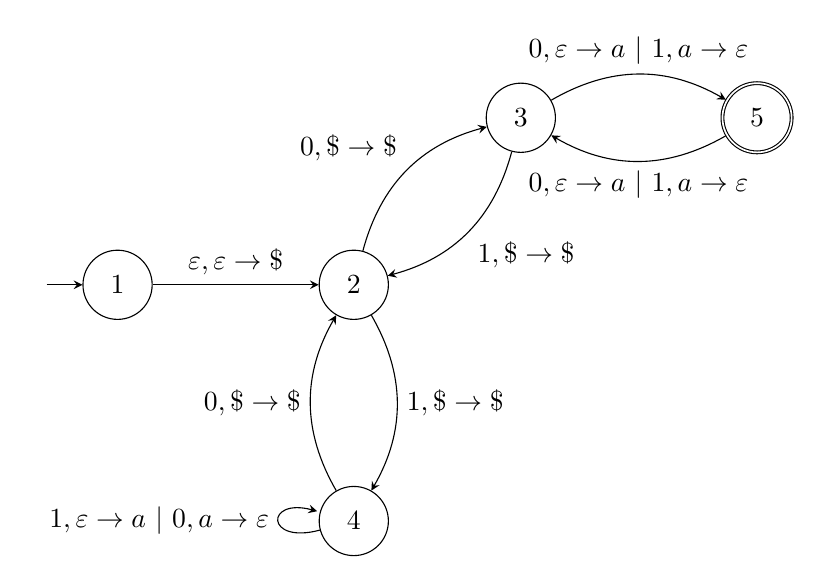
\begin{tikzpicture}[%
    >=stealth,
    node distance=3cm,
    on grid,
    auto
    ]

    \node[initial,initial text=,state] (1)  {1};
    \node[state] (2) [right of=1] {2};
    \node[state] (3) [above right of=2] {3};
    \node[state] (4) [below of=2] {4};
    \node[state, accepting] (5) [right of=3] {5};

    \path[->] (1) edge node {$\varepsilon, \varepsilon \rightarrow \$$} (2);
    \path[->] (2) edge[bend left] node {$0, \$ \rightarrow \$$} (3);
    \path[->] (3) edge[bend left] node {$1, \$ \rightarrow \$$} (2);
    \path[->] (3) edge[bend left] node {$0,\varepsilon \rightarrow a\ |\ 1, a \rightarrow \varepsilon$} (5);
    \path[->] (5) edge[bend left] node {$0,\varepsilon \rightarrow a\ |\ 1, a \rightarrow \varepsilon$} (3);
    \path[->] (2) edge[bend left] node {$1, \$ \rightarrow \$$} (4);
    \path[->] (4) edge[bend left] node {$0, \$ \rightarrow \$$} (2);

    \path[->] (4) edge[loop left] node {$1, \varepsilon \rightarrow a\ |\ 0, a \rightarrow \varepsilon$} (4);


    \end{tikzpicture}

\item The compliment of $C = \{ww | w\in \Sigma^*\}$ over the alphabet $\Sigma = \{0,1\}$. (10 Points)

    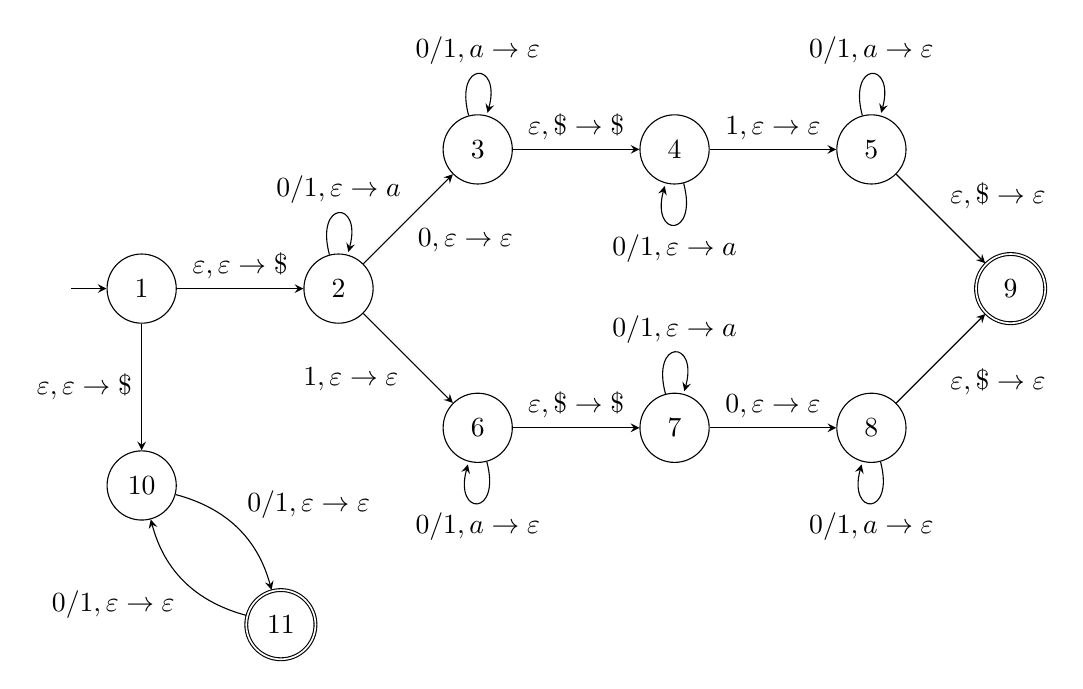
\begin{tikzpicture}[%
    >=stealth,
    node distance=2.5cm,
    on grid,
    auto
    ]

    \node[initial,initial text=,state] (1)  {1};
    \node[state] (2) [right of=1] {2};
    \node[state] (3) [above right of=2] {3};
    \node[state] (4) [right of=3] {4};
    \node[state] (5) [right of=4] {5};
    \node[state] (6) [below right of=2] {6};
    \node[state] (7) [right of=6] {7};
    \node[state] (8) [right of=7] {8};
    \node[state, accepting] (9) [above right of=8] {9};
    \node[state] (10) [below of=1] {10};
    \node[state, accepting] (11) [below right of=10] {11};

    \path[->] (1) edge node {$\varepsilon, \varepsilon \rightarrow \$$} (2);
    \path[<-] (3) edge node {$0, \varepsilon \rightarrow \varepsilon$} (2);
    \path[<-] (6) edge node {$1, \varepsilon \rightarrow \varepsilon$} (2);
    \path[->] (3) edge node {$\varepsilon, \$ \rightarrow \$$} (4);
    \path[->] (4) edge node {$1,\varepsilon \rightarrow \varepsilon$} (5);
    \path[->] (5) edge node {$\varepsilon, \$ \rightarrow \varepsilon$} (9);
    \path[->] (6) edge node {$\varepsilon, \$ \rightarrow \$$} (7);
    \path[->] (7) edge node {$0,\varepsilon \rightarrow \varepsilon$} (8);
    \path[<-] (9) edge node {$\varepsilon, \$ \rightarrow \varepsilon$} (8);
    \path[<-] (10) edge node {$\varepsilon, \varepsilon \rightarrow \$$} (1);
    \path[->] (10) edge[bend left] node {$0/1, \varepsilon \rightarrow \varepsilon$} (11);
    \path[->] (11) edge[bend left] node {$0/1, \varepsilon \rightarrow \varepsilon$} (10);

    \path[->] (2) edge[loop above] node {$0/1, \varepsilon \rightarrow a$} (2);
    \path[->] (3) edge[loop above] node {$0/1, a \rightarrow \varepsilon$} (3);
    \path[->] (4) edge[loop below] node {$0/1, \varepsilon \rightarrow a$} (4);
    \path[->] (5) edge[loop above] node {$0/1, a \rightarrow \varepsilon$} (5);
    \path[->] (6) edge[loop below] node {$0/1, a \rightarrow \varepsilon$} (6);
    \path[->] (7) edge[loop above] node {$0/1, \varepsilon \rightarrow a$} (7);
    \path[->] (8) edge[loop below] node {$0/1, a \rightarrow \varepsilon$} (8);

    \end{tikzpicture}

\end{enumerate}

\newpage


\subsection*{Problem 5}
    Recall that in our definition of a PDA, the transition function was described as $\delta: Q\times\Sigma_\varepsilon\times\Gamma_\varepsilon\to\mathcal{P}(Q\times\Gamma_\varepsilon)$. In an attempt to advance the human knowledge in the field of theoretical computer science, Professor Professorson has introduced a new concept, an extended pushdown automaton (EPDA).

    An EPDA is defined in the same way as a PDA, except for the transition function component, which is now given as $\delta: Q\times\Sigma_\varepsilon\times\Gamma_\varepsilon\to\mathcal{P}(Q\times\Gamma^*)$. In other words, an EPDA can push a string of multiple characters onto the stack in a single transition. 

    Professor Professorson believes that EPDAs are equivalent to PDAs (and thus to CFGs), but are easier to construct. If true, his idea can revolutionize the industry of PDA generation.
\begin{enumerate}[(a)]
    \item Prove the professor wrong. In fact, show that for \textit{any} language
    $L\subseteq\Sigma^*$, some EPDA recognizes it. (10 Points)

    The probem with the EPDA is in the transition function. The transition function given allows
    for infinite number of transitions because $\mathcal{P}(Q \times \Gamma^*)$ is infinite.
    This allows us to have our EPDA recognize an infininte number of strings by first pushing
    them on the stack in reverse. Then to process the input string we can have transitions
    that read the input string and pop off only matching symbols on the stack. If we reach the
    bottom of the stack and can pop off a $\$$ the EPDA accepts.

    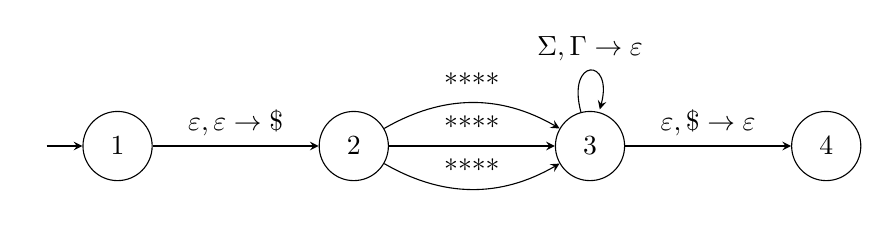
\begin{tikzpicture}[%
    >=stealth,
    node distance=3cm,
    on grid,
    auto
    ]

    \node[initial,initial text=,state] (1)  {1};
    \node[state] (2) [right of=1] {2};
    \node[state] (3) [right of=2] {3};
    \node[state] (4) [right of=3] {4};

    \path[->] (1) edge node {$\varepsilon, \varepsilon \rightarrow \$$} (2);
    \path[->] (3) edge[loop above] node {$\Sigma, \Gamma \rightarrow \varepsilon$} (4);
    \path[->] (2) edge[bend left] node {****} (3);
    \path[->] (2) edge node {****} (3);
    \path[->] (2) edge[bend right] node {****} (3);
    \path[->] (3) edge node {$\varepsilon, \$ \rightarrow \varepsilon$} (4);

    \end{tikzpicture}

    **** represents an infinite number of transitions that push all strings in the language
    in reverse order.
    NOTE: In the picture above $\Sigma, \Gamma \rightarrow \varepsilon$ represents every
    transition for each $a \in \Sigma$ and $b \in \Gamma$ such that $a = b$.

    \item Shocked by our previous result, the professor claims that he can prove the equivalence
    of EPDAs and PDAs. Actually, we have already used the shorthand notation for pushing an
    entire string onto the stack in the proof of the PDA--CFG equivalence theorem.

    For example, any transition of the form $(r,xyz) \in \delta(q,a,s)$ can be rewritten as a
    series of one-character transitions by adding extra states:
    $(q_1,x)\in\delta(q,a,s)$, $\delta(q_1,\varepsilon,\varepsilon)=
    \{(q_2,y)\}$, $\delta(q_2,\varepsilon,\varepsilon)=\{(r,z)\}$ (for more details and a
    picture, see the lecture notes or Sipser, pages 116--117).

    According to Professor Professorson, this allows us to convert any EPDA into an equivalent
    PDA. Explain how this construction does not contradict the existence of non-context free
    languages. (5 Points)\\

    We have shown in part a that an EPDA can have an infinite number of transitions.
    Now consider the non-context free language (as we proved in class):\\
    \[L=\{0^n1^n2^n | n \geq 0\} \]
    In order to construct an EPDA that recognizes $L$ we need to have an infinite number of
    transitions because $n$ is unbounded. In order to convert this to a PDA we will need
    an infinite number of states because each transition will be converted to multiple states
    as per the conversion proposed above.
    But this violates the definition of a PDA having a finite set of states. Therefore an EPDA
    is not equivalent to a PDA. Additionally since we cannot convert the EPDA to a true PDA
    that recognizes $L$, it must be the case there there are non context free languages.
    \[ \square \]


\end{enumerate}

\newpage


\subsection*{Problem 6}
Consider grammar $G = (\{$S,A,B$\},\{0,1\}$,R,S), where
\[
    S \rightarrow AB\ |\ BA
\]
\[
    A \rightarrow 0\ |\ 0A0\ |\ 0A1\ |\ 1A0\ |\ 1A1 \\
\]
\[
    B \rightarrow 1\ |\ 0B0\ |\ 0B1\ |\ 1B0\ |\ 1B1 \\
\]

\begin{enumerate}[(a)]
\item What language does this grammar generate? Give a simple description with little
or no mathematical notation (no more than 15-20 words). (7 Points)

G is the set of all pairs of strings of odd length, who's central symbols are different,
concatenated together.

\item Prove your answer to part (a). That is, prove that every string of the language
can be derived in G, and that every string that can be derived is in the language. (10 Points)

%TODO
\textbf{String to grammar:}\\
Move through the string keeping track of the symbols in the center. When you find two symbols
that differ, mark them. If the central symbol on the left is a 0, then $S \rightarrow AB$
otherwise if the central symbol on the left is a 1, then $S \rightarrow BA$. Now we have two
strings that are of odd length separated. To produce the grammar further we look at the symbols
to the left and right in each string recursivly. We have 4 cases:\\
(Let X in the following be A or B for each respective string.)
\begin{enumerate}[1.]
\item If the outer string is 0X0
\item If the outer string is 1X0
\item If the outer string is 0X1
\item If the outer string is 1X1
\end{enumerate}

For each of these cases we have rules in for each variable in the grammer.\\
Therefore we can go from a string to the grammar.

\textbf{Grammar to string:}\\
Since we have production rules that lead to a single terminal: $A \rightarrow 0$ and
$B \rightarrow 1$, \\
Or two terminals with a single variable:
$B \rightarrow 0B0\ |\ 1B1\ |\ 1B0\ |\ 0B1$ and , $B \rightarrow 0B0\ |\ 1B1\ |\ 1B0\ |\ 0B1$
we are left with strings that are odd length.

$S \rightarrow AB\ |\ BA$ allows us to concatenate the two strings together.\\
Since the final terminals from $A$ and $B$ are different, we will have central symbols in each
string that are different.

Therefore we are left with pairs of strings, who's central symbols are different, concatenated
together.

\item Is G ambiguous? If your answer is yes", give an example of a string with 2
different derivations. (3 Points)

Yes: \\
$S \Rightarrow AB \Rightarrow 0A0B \Rightarrow 000B \Rightarrow
0001B1 \Rightarrow 000111$ \\
and \\
$S \Rightarrow AB \Rightarrow 0A1B \Rightarrow 00A11B \Rightarrow
00011B \Rightarrow 000111$
\end{enumerate}

\end{document}
